\documentclass[10pt,a4paper]{beamer}

\usepackage[utf8]{inputenc}
\usepackage[russian]{babel}
\usepackage[OT1]{fontenc}
\usepackage{amsmath}
\usepackage{amsfonts}
\usepackage{amssymb}
\usepackage{makeidx}
\usepackage{graphicx}
\usepackage{xcolor}
\usepackage{multirow}

\titlegraphic{
   
\includegraphics[width=4cm]{images/sfera.jpg}
}

\author{Николай Анохин \and Михаил Фирулик}
\title{Введение в Data Science \\ Занятие 2. Линейные модели}

\beamertemplatenavigationsymbolsempty

\begin{document}

\maketitle

\logo{
    
\includegraphics[width=4cm,keepaspectratio]{images/sfera.jpg}\hspace{0.45em}
}

% ============================================== %

\begin{frame}{Где мы находимся (глобально)}

\begin{center}
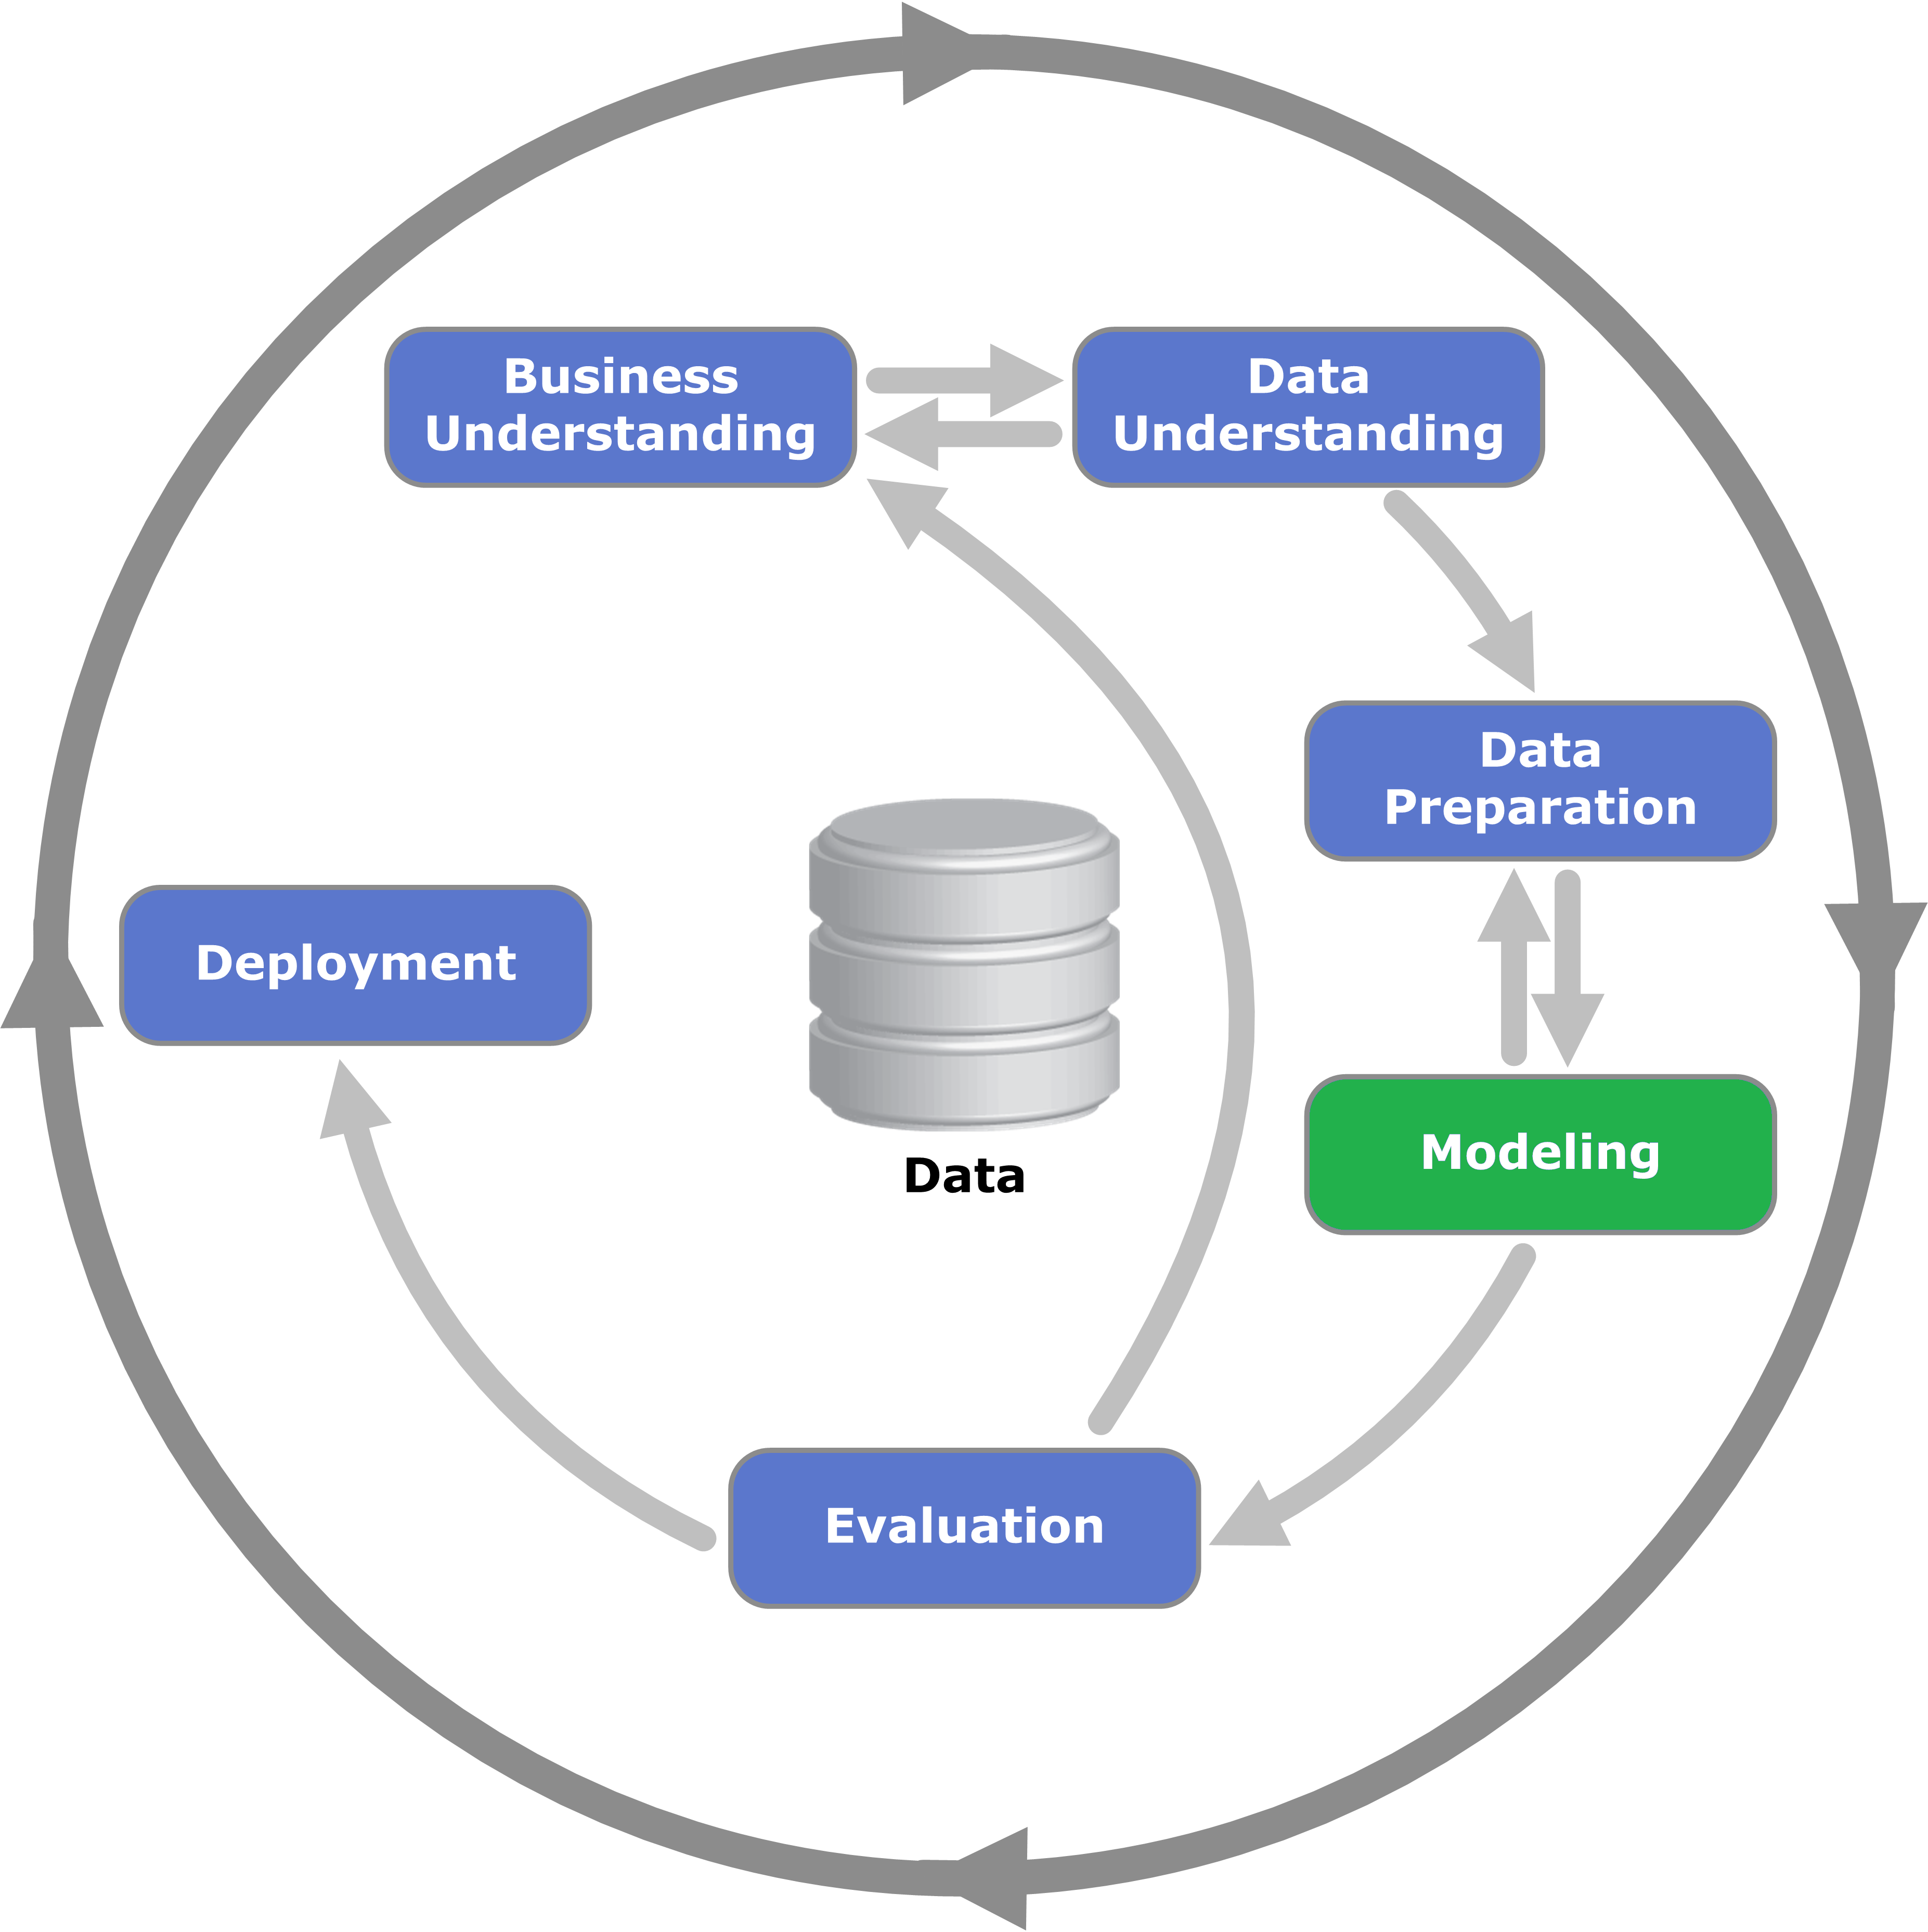
\includegraphics[scale=0.4]{images/crisp.png}
\end{center}

\end{frame}

% ============================================== %

\begin{frame}{Где мы находимся (локально)}

\begin{enumerate}

\item[M] {\color{gray} Выдвигаем гипотезу насчет {\bf модели} - семейства параметрических функций вида
\[
Y = \{ y(x, \theta) : X \times \Theta \rightarrow T \},
\]
которая могла бы решить нашу задачу (model selection)}

\item[L] {Выбираем наилучшие параметры модели $\theta^*$, используя {\bf алгоритм обучения}
\[
A(\boldsymbol X, \boldsymbol T) : (X, T)^N \rightarrow Y
\]
(learning/inference)}

\item[D] {\color{gray} Используя полученную модель $y^*(x) = y(x, \theta^*)$, классифицируем неизвестные объекты (decision making)}

\end{enumerate}

\end{frame}

% ============================================== %

\begin{frame}{Как выбрать параметры модели?}

Решить задачу оптимизации, чтобы получить значения $\theta^*$ 
\vspace{1em}

Варианты подходов
\begin{itemize}
\item $\theta$ -- фиксировано, но неизвестно: ищем $\theta$, согласующееся с обучающей выборкой
\item $\theta$ -- случайная величина, распределенная по известному закону: ищем параметры распределения
\end{itemize}

\end{frame}

% ============================================== %

\begin{frame}

\tableofcontents

\end{frame}

% ============================================== %

\section{Обобщенные линейные модели}

% ============================================== %

\begin{frame}{8 марта (is coming)}

\begin{center}
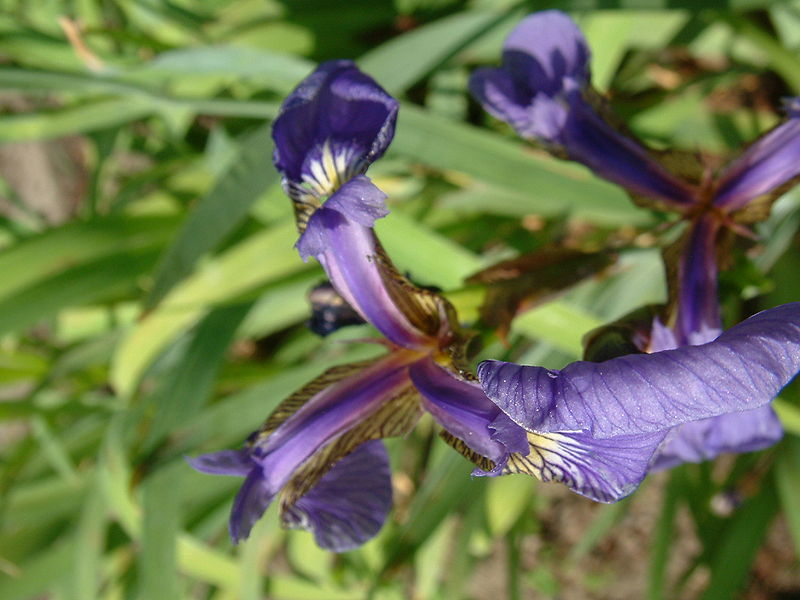
\includegraphics[scale=0.1]{images/setosa.jpg} \;
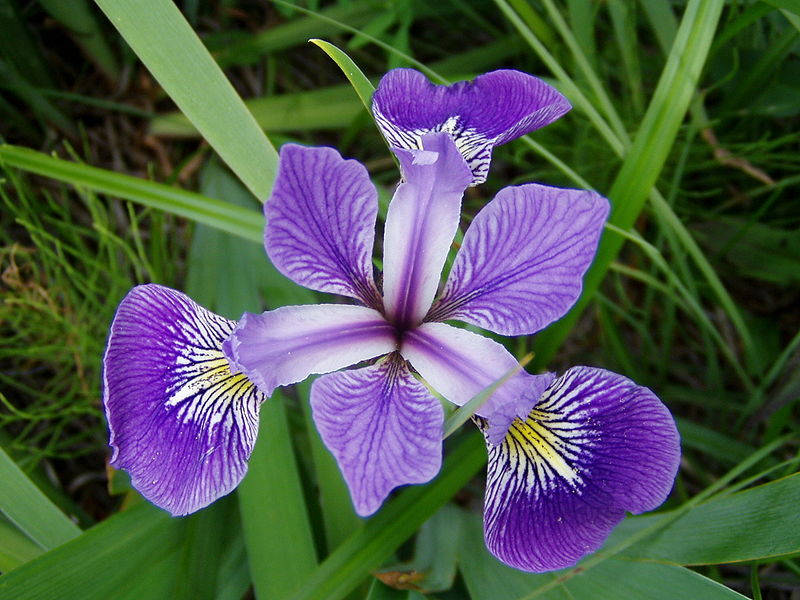
\includegraphics[scale=0.1]{images/versicolor.jpg} \;
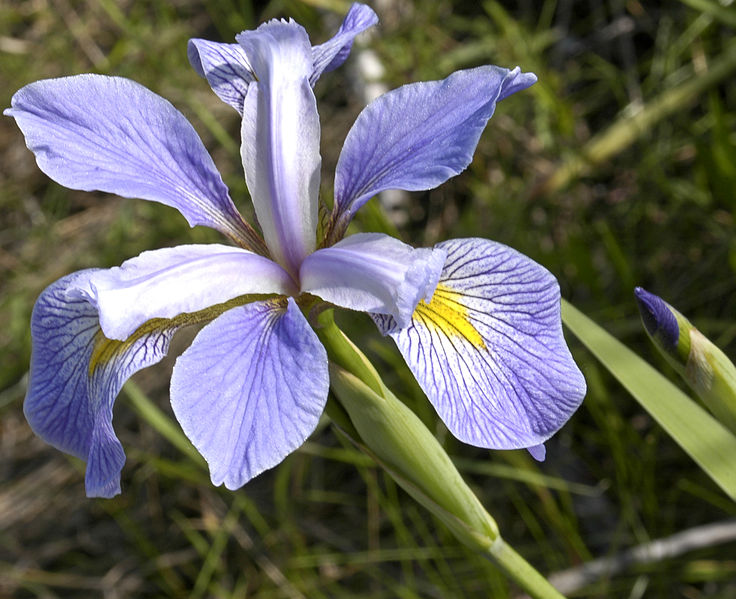
\includegraphics[scale=0.416]{images/virginica.jpg}
\end{center}
{\large \hspace{4.5em} Setosa \hspace{3.3em} Versicolor \hspace{2.5em} Virginica}

\begin{exampleblock}{Задача}
Определить вид ириса на основании длины чашелистика, ширины чашелистика, длины лепестка и ширины лепестка.
\end{exampleblock}

\end{frame}

% ============================================== %

\begin{frame}{Ирисы Фишера}

\begin{center}
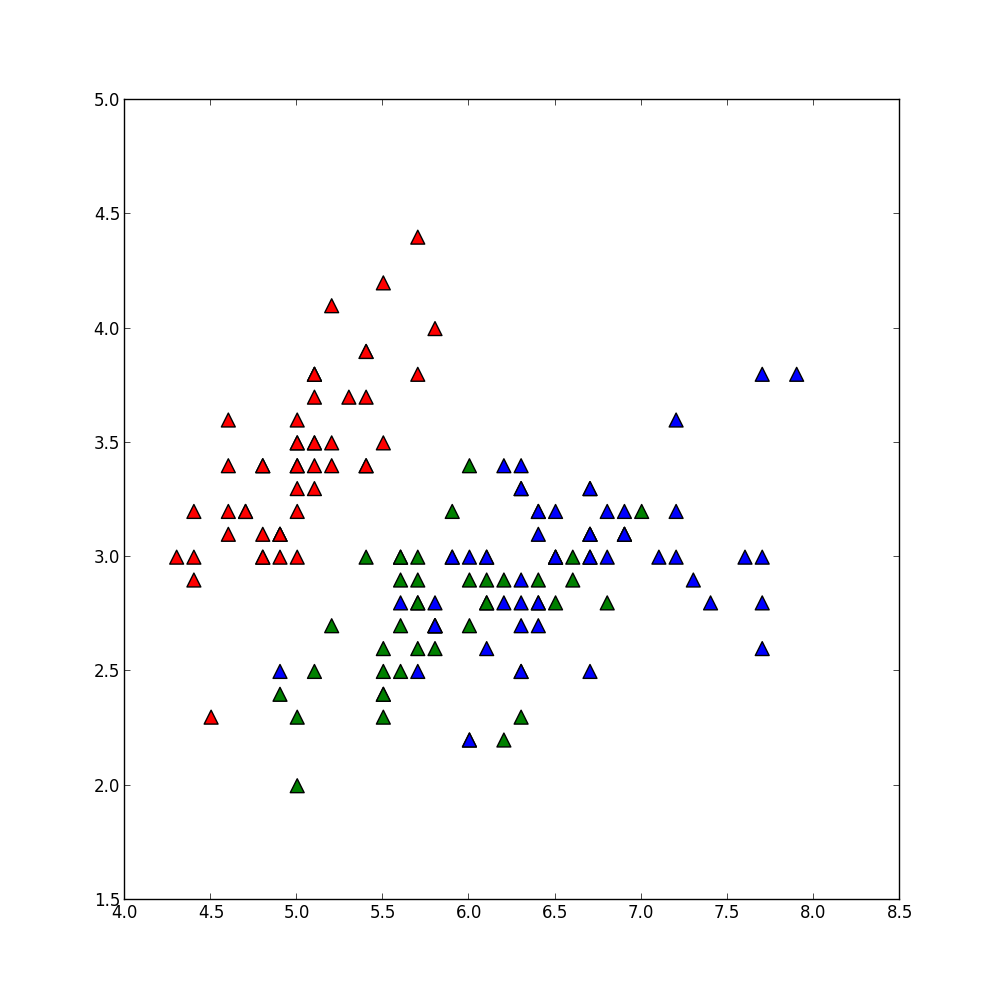
\includegraphics[scale=0.2]{images/iris01.png} \;
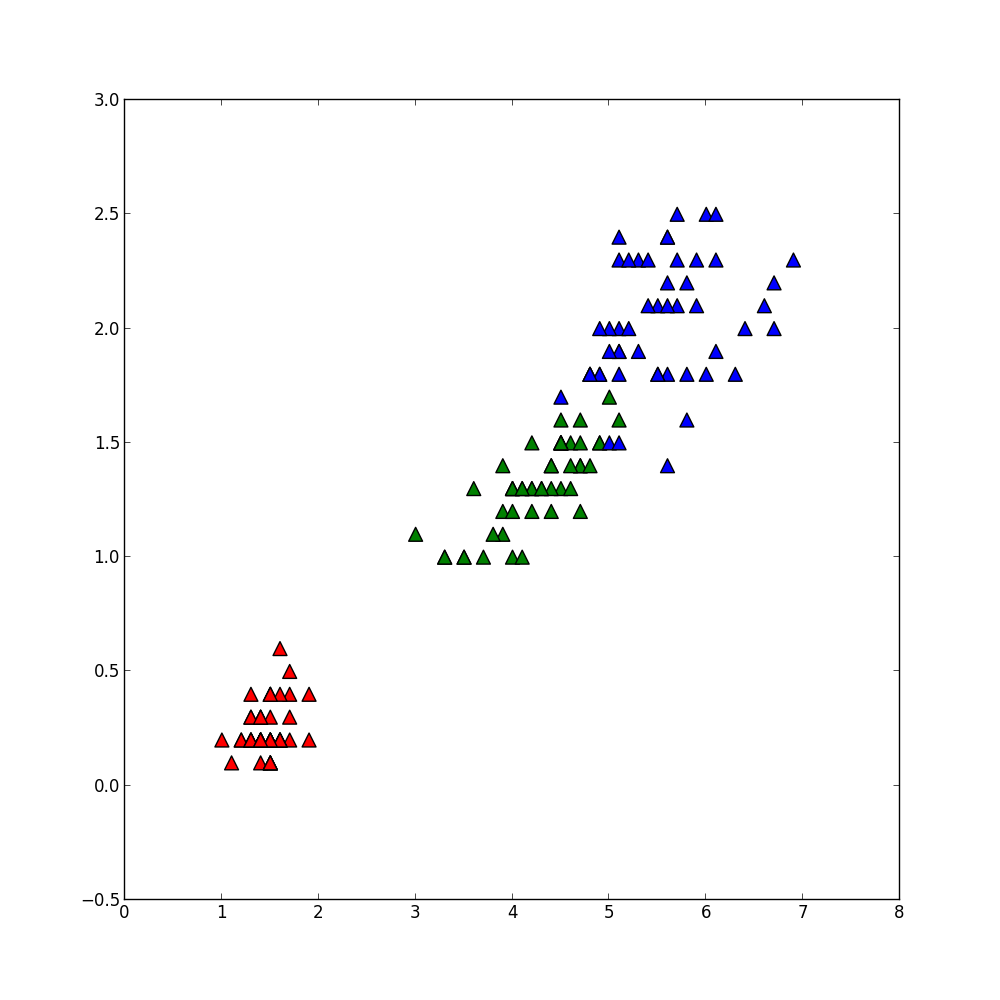
\includegraphics[scale=0.2]{images/iris23.png}
\end{center}

\end{frame}

% ============================================== %

\begin{frame}{Линейные модели}

\begin{columns}[T]
    \begin{column}{.5\textwidth}
	Рассматривается случай 2 классов
	\vspace{0.3em} 
    
    Функция принятия решения
    \[
    y(\mathbf{x}) = \mathbf{w}^\top \mathbf{x} + w_0
    \]
    Регионы принятия решения
    \[
    R_1 = \{\mathbf{x}\,:\,y(\mathbf{x}) > 0\}
    \]
    \[
    R_2 = \{\mathbf{x}\,:\,y(\mathbf{x}) < 0\}
    \]
    Задача
    
    найти параметры модели $\mathbf{w}$, $w_0$
    \end{column}
       
    \begin{column}{.5\textwidth}
    \vspace{-0em}
	\begin{center}
   		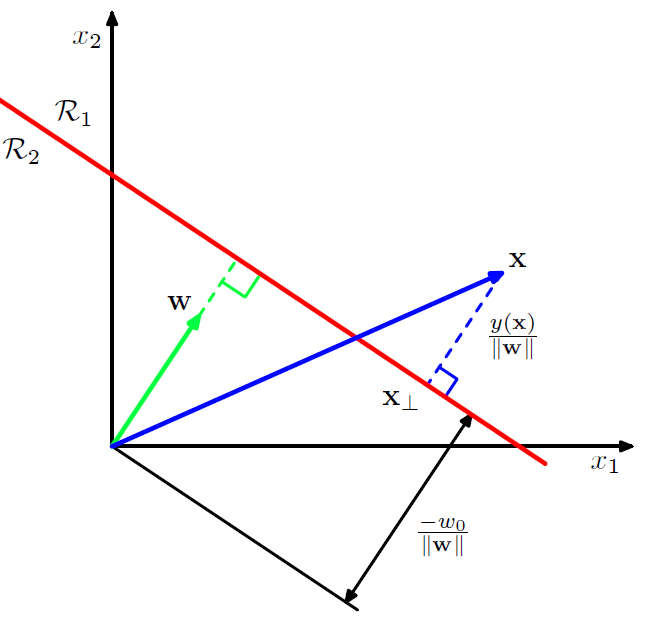
\includegraphics[scale=0.3]{images/linear.png}
    \end{center}
    \end{column}
  \end{columns}

\end{frame}

% ============================================== %

\begin{frame}{Линейные модели: наблюдения}

\begin{columns}[T]
    \begin{column}{.5\textwidth}
	Разделяющая поверхность
	\vspace{0.3em}
	\[
	\mathcal{D} = \{\mathbf x\,:\,\mathbf w^\top \mathbf x + w_0 = 0\}
	\]	
	
	\begin{enumerate}	
	\item $\mathbf{w}$ -- нормаль к $\mathcal{D}$
	
	\item $d = -\frac{w_0}{\|\mathbf{w}\|}$ -- расстояние от центра координат до $\mathcal{D}$
	
	\item $r(\mathbf{x}) = \frac{y(x)}{\|\mathbf{w}\|}$ -- расстояние от $\mathcal{D}$ до $\mathbf{x}$	
	\end{enumerate}
	
	Положим $x_0 \equiv 1$, получим модель
	\[
	y(\tilde{\mathbf{x}}) = \tilde{\mathbf w}^\top \tilde{\mathbf{x}}
	\] 
    
    \end{column}
       
    \begin{column}{.5\textwidth}
    \vspace{-0em}
	\begin{center}
   		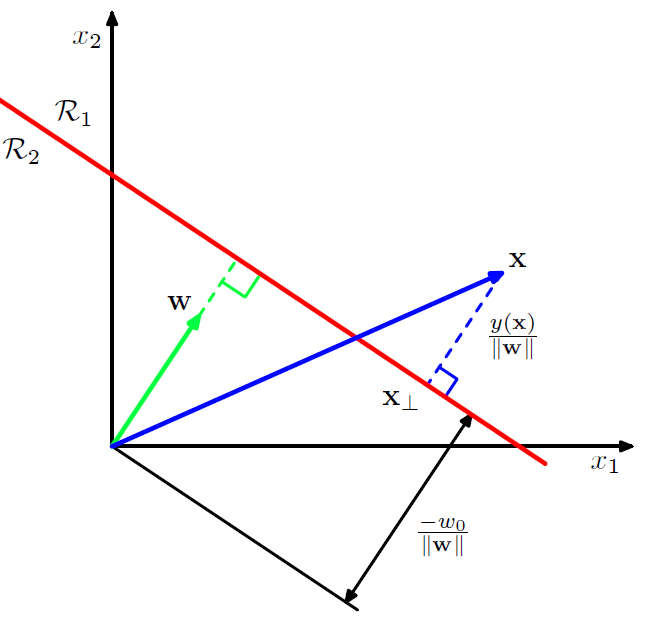
\includegraphics[scale=0.3]{images/linear.png}
    \end{center}
    \end{column}
  \end{columns}

\end{frame}

% ============================================== %

\begin{frame}{Обобщенные линейные модели}

Линейная модель
\[
y(\mathbf{x}) = w_0 + \sum w_i x_i
\]
Квадратичная модель
\[
y(\mathbf{x}) = w_0 + \sum w_i x_i + \sum \sum w_{ij} x_i x_j
\]
Обобщенная линейная модель
\[
g(\mathbf{x}) = \sum a_i \phi_i(\mathbf{x}) = \mathbf{a}^\top \mathbf{y}
\]

\end{frame}

% ============================================== %

\begin{frame}{Случай линейно разделимых классов}

Обобщенная линейная модель
\[
g(\mathbf{x}) = \sum a_i \phi_i(\mathbf{x}) = \mathbf{a}^\top \mathbf{y}
\]
Дана обучающая выборка $\mathbf{Y} = \{\mathbf{y}_1, \ldots, \mathbf{y}_N\}$

\begin{center}
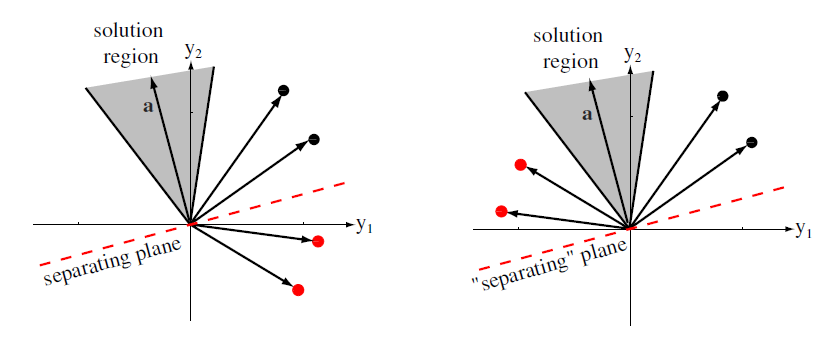
\includegraphics[scale=0.35]{images/optimzation.png}
\end{center}

\begin{exampleblock}{Идея}
Преобразовать объекты второго класса в обратные им и решать задачу оптимизации в области $a^T \mathbf{y}_i > 0, \; \forall i$
\end{exampleblock}

\end{frame}

% ============================================== %

\begin{frame}{Задача оптимизации}

\begin{block}{Задача}
Минимизируем критерий $J(a)$ при условиях $a^T \mathbf{y}_i > 0, \; \forall i$
\end{block}

Пусть $\mathcal{Y}$ -- множество неправильно проклассифицированных объектов
\begin{itemize}
\item $J_e(a) = \sum_{\mathbf{y} \in \mathcal{Y}} 1$ 
\item $J_p(a) = \sum_{\mathbf{y} \in \mathcal{Y}} - a^\top \mathbf{y}$ 
\item $J_q(a) = \sum_{\mathbf{y} \in \mathcal{Y}} (a^\top \mathbf{y})^2$
\item $J_r(a) = \sum_{\mathbf{y} \in \mathcal{Y}} \frac{(a^\top \mathbf{y})^2 - b}{\|\mathbf{y}\|}$
\end{itemize}
Улучшение: добавить отступы

\end{frame}

% ============================================== %

\begin{frame}{Градиентный спуск}


\texttt{1. initialise $a$, $J(a)$, $\eta(k)$, $\epsilon$, $k=0$}

\texttt{2. \;\; do $k \leftarrow k + 1$}

\texttt{3. \;\;\;\; $a \leftarrow a - \eta(k) \nabla J(a) $}

\texttt{4. \;\; until $\eta(k) \nabla J(a)$ < $\epsilon$}

\texttt{5. return a}

\texttt{5. end}

\vspace{0.5em}

\end{frame}

% ============================================== %

\begin{frame}{Инкрементальный алгоритм}

Рассматриваем $J_r(a) = \sum_{y \in \mathcal{Y}} \frac{(a^\top \mathbf{y})^2 - b}{\|y\|}$
\vspace{1em}

\texttt{1. initialise $a$, $\eta(k)$, $k=0$}

\texttt{2. \;\; do $k \leftarrow k + 1$}

\texttt{3. \;\;\;\; if $\mathbf{y}_k$ is misclassified $a \leftarrow a - \eta(k)\frac{(a^\top \mathbf{y_k})^2 - b}{\|\mathbf{y}_k\|^2} \mathbf{y}_k $}

\texttt{4. \;\; until no errors left}

\texttt{5. return a}

\texttt{6. end}

\vspace{0.5em}

\end{frame}

% ============================================== %

\begin{frame}{Случай линейно неразделимых классов}

\begin{itemize}
\item Использовать $\eta(k) \rightarrow 0$ при $k \rightarrow \infty$
\item От системы неравенств перейти к системе линейных уравнений
\item Линейное программирование
\end{itemize}

\end{frame}

% ============================================== %

\begin{frame}{Снова переобучение}

Оптимизируем критерий с регуляризацией
\[
J_1(a) = J(a) + \lambda J_R(a)
\]
$\lambda$ -- коэффициент регуляризации
\[
J_R(a) = \sum |a_j|^q
\]
\begin{center}
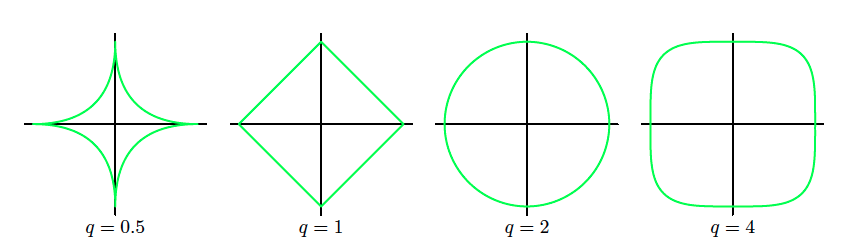
\includegraphics[scale=0.3]{images/regularization.png}
\end{center}

\end{frame}

\begin{frame}{Перцептрон: результаты}

	\begin{center}
   		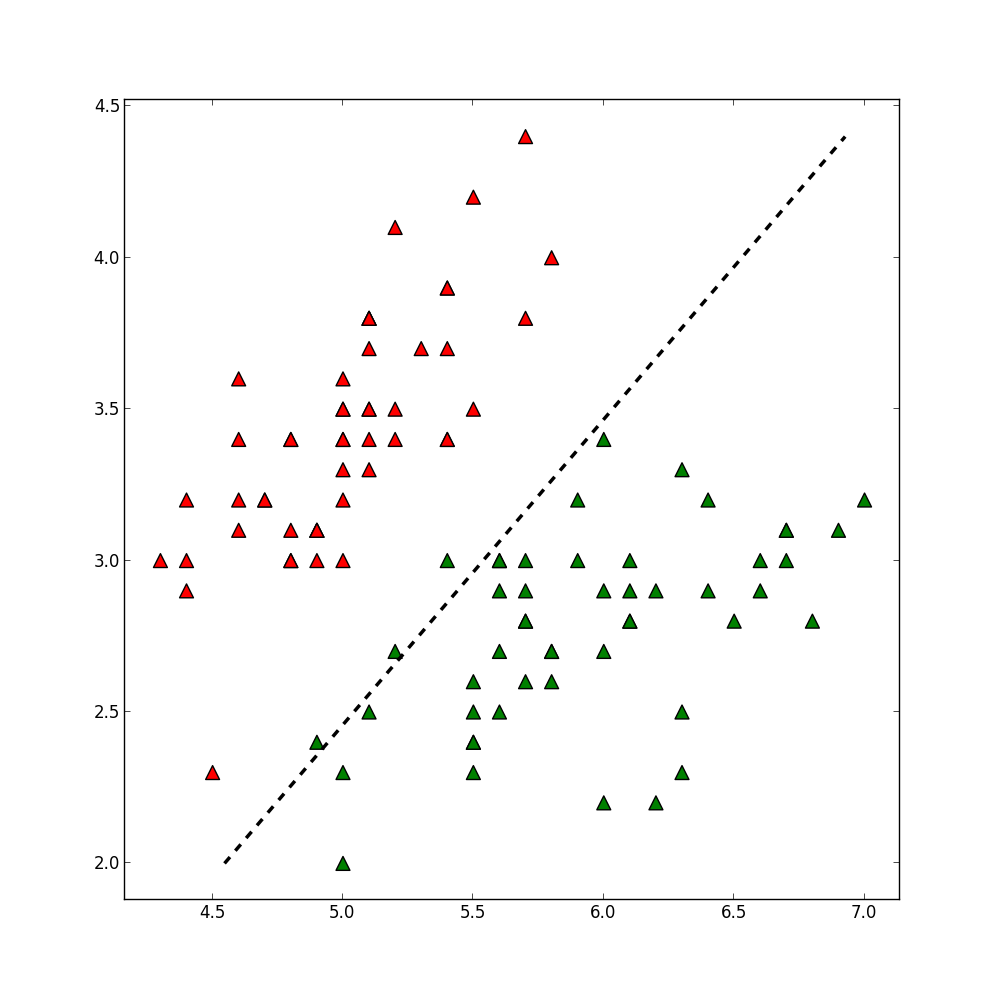
\includegraphics[scale=0.2]{images/perc01.png}\;   		
   		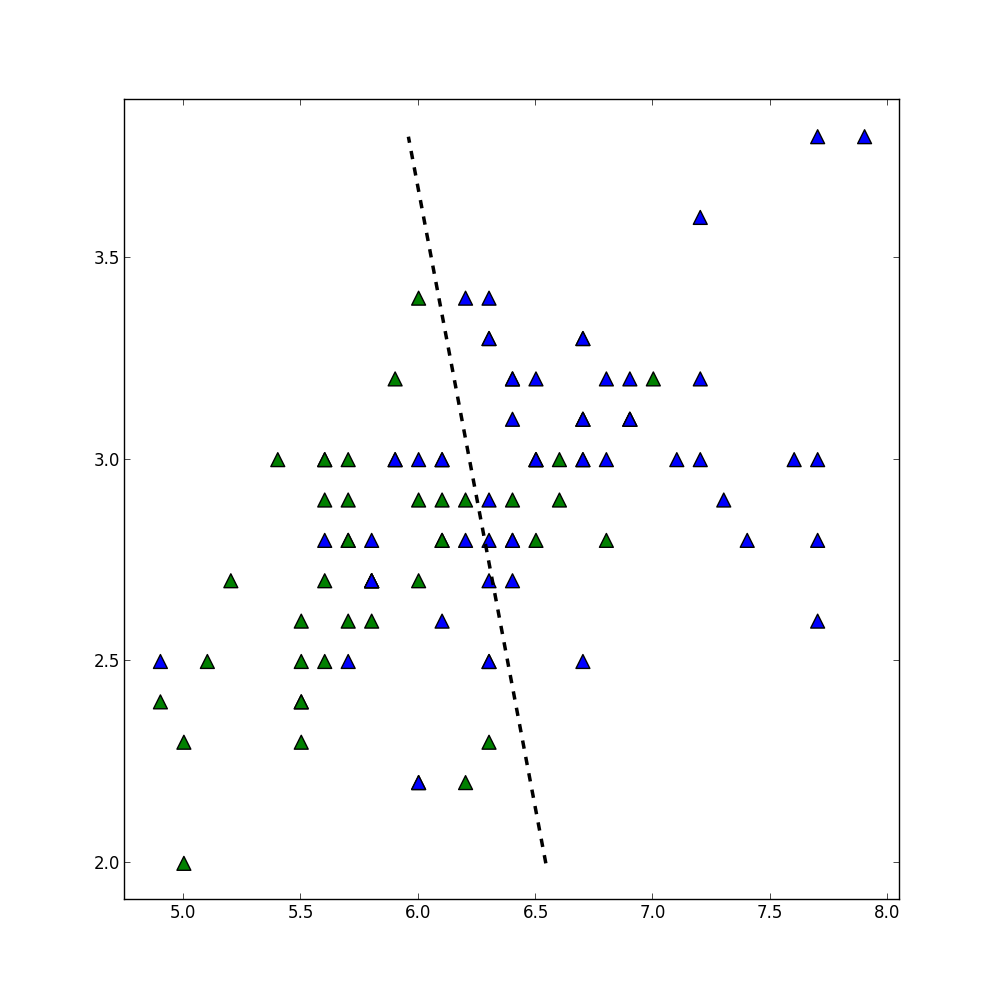
\includegraphics[scale=0.2]{images/perc12.png}
    \end{center}

\end{frame}

% ============================================== %

\section{Метод максимального правдоподобия}

% ============================================== %

\begin{frame}{Метод максимального правдоподобия}

\begin{block}{Задача}
Дана обучающая выборка $\mathbf{X}$. Предполагая, что распределение $p(\mathbf{x} | \theta)$ известно, найти значения параметров $\theta$.
\end{block}

\vspace{1em}
Интуиция: найти такие $\theta$, которые максимизируют вероятность $P(\mathbf{X}|\theta)$.

\vspace{1em}
При предположении, что обучающие образцы независимы, имеем	
\[
P(\mathbf{X} | \theta) = \prod p(\mathbf{x}_i | \theta)
\]
Функция правдоподобия
\[
l(\theta) = \log{P(\mathbf{X} | \theta)} = \sum \log p(\mathbf{x}_i | \theta)
\]
Требуется найти
\[
\theta = \arg \max_\theta l(\theta)
\]

\end{frame}

% ============================================== %

\begin{frame}{Нормальное распределение}

\[
p(x | \mu) = \frac{1}{\sigma \sqrt{2 \pi}} e^{-\frac{(x-\mu)^2}{2\sigma^2}}
\]

\begin{exampleblock}{Задача}
Дана выборка $\mathbf{X}$ объектов $x$, распределенных согласно одномерному нормальному закону $N(\mu, \sigma^2)$. Используя принцип максимального правдоподобия, оценить значение $\mu$ при известном значении $\sigma$.
\end{exampleblock}

\end{frame}

% ============================================== %

\begin{frame}{Вероятностная линейная модель}

Рассматриваем 2 класса
\[
p(C_1 | x) = \frac{p(x | C_1)p(C_1)}{p(x | C_1)p(C_1) + p(x | C_2)p(C_2)} = \frac{1}{1 + e^{-a}} = \sigma(a)
\]
\[
a = \ln \frac{p(x | C_1)p(C_1)}{p(x | C_2)p(C_2)}
\]
$\sigma(a)$ -- сигмоид-функция, $a = \ln (\sigma/(1-\sigma))$

\begin{center}
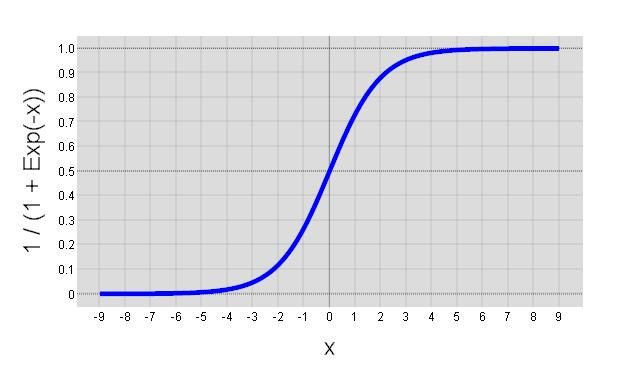
\includegraphics[scale=0.3]{images/sigmoid.jpg}
\end{center}

Упражнение: $p(\mathbf{x} | C_k) = \mathcal{N}(\mathbf{\mu}_k, \mathbf{\Sigma})$. Проверить, что $p(C_k | x) = \sigma(\mathbf{w}^\top \mathbf{x} + w_0)$

\end{frame}

% ============================================== %

\begin{frame}{(Еще более) обобщенная линеная модель}

\begin{columns}[T]
    \begin{column}{.5\textwidth}
    \vspace{2em}
	Базисные функции $\phi_n(\mathbf{x})$
\[
\phi_n(\mathbf{x}) = \exp\left[ -\frac{(x - \mu_n)^2}{2 s^2}\right]
\]
Функция активации $f(a)$
\[
f(a) = \sigma(a)
\]
(Совсем) обобщенная линейная модель
\[
y(\mathbf{x}, \mathbf{w}) = f(\mathbf{w}^\top \phi(\mathbf{x}))
\]

    \end{column}
       
    \begin{column}{.5\textwidth}
    \vspace{-2em}
	\begin{center}
   		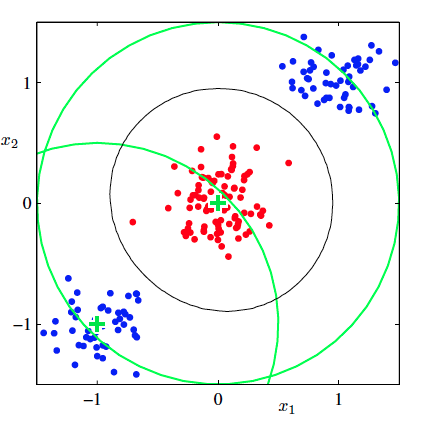
\includegraphics[scale=0.25]{images/nl.png}
   		
   		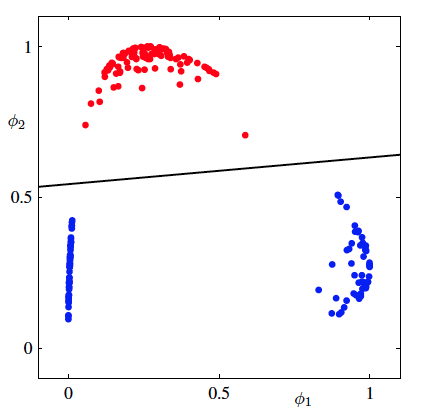
\includegraphics[scale=0.25]{images/l.png}
    \end{center}
    \end{column}
  \end{columns}

\end{frame}

% ============================================== %

\begin{frame}{Логистическая регрессия}

дано
\[
\{\phi_n = \phi(\mathbf{x}_n), t_n\}, \; t_n \in \{ 0,1\}, \; n = 1 \ldots N
\]
модель
\[
p(C_1 | \phi) = y(\phi) = \sigma(\mathbf{w}^\top \phi)
\]
функция правдоподобия
\[
l(\mathbf{w}) = \log \left[ \prod_{n=1}^N p^{t_n}(C_1 | \phi_n) (1 - p(C_1 | \phi_n))^{1 - t_n}\right] = 
\]
\[
= \sum_{n=1}^N {t_n \log p(C_1 | \phi_n) + (1- t_n) \log (1 - p(C_1 | \phi_n))} = - J_e(\mathbf{w}) 
\]
градиент
\[
\nabla J_e(\mathbf{w}) = \sum_{n=1}^N (p(C_1 | \phi_n) - t_n) \phi_n \rightarrow min_{\mathbf{w}}
\]

\end{frame}

% ============================================== %

\begin{frame}{Логистическая регрессия: результаты}

	\begin{center}
   		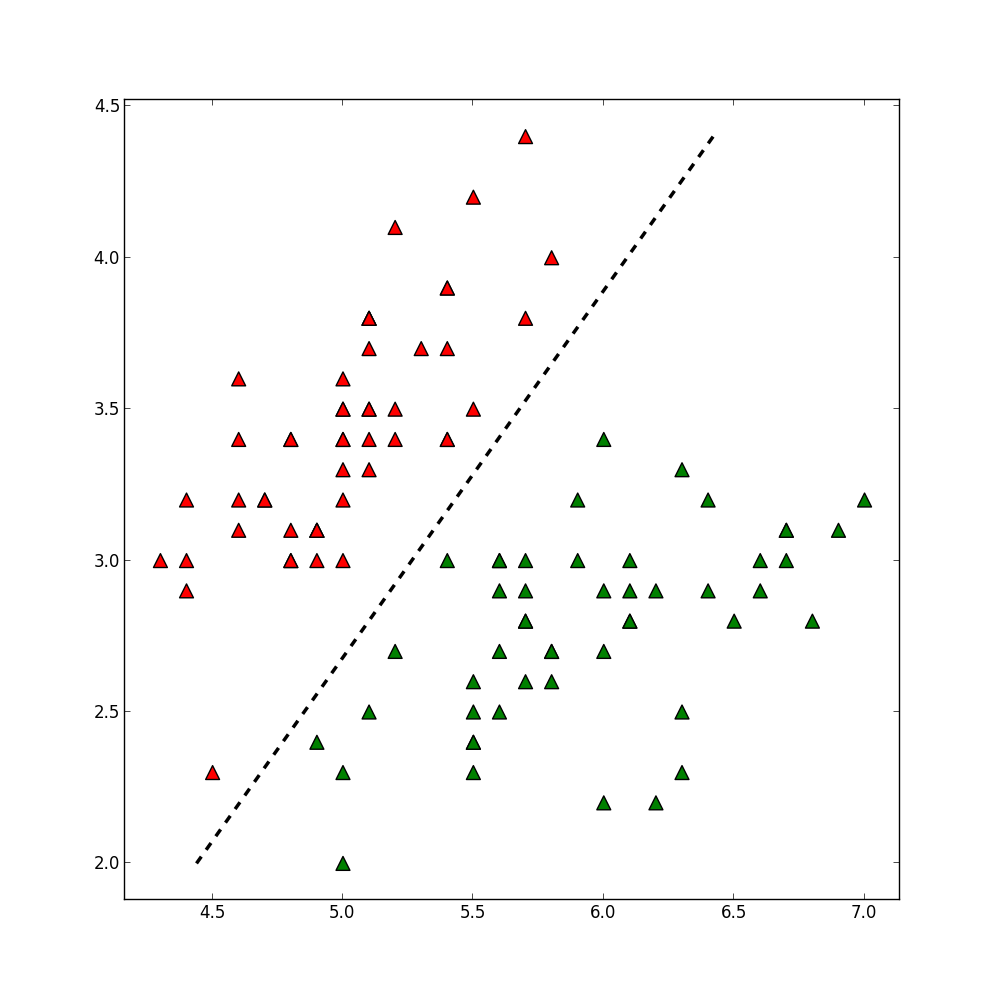
\includegraphics[scale=0.2]{images/lr01.png}\;   		
   		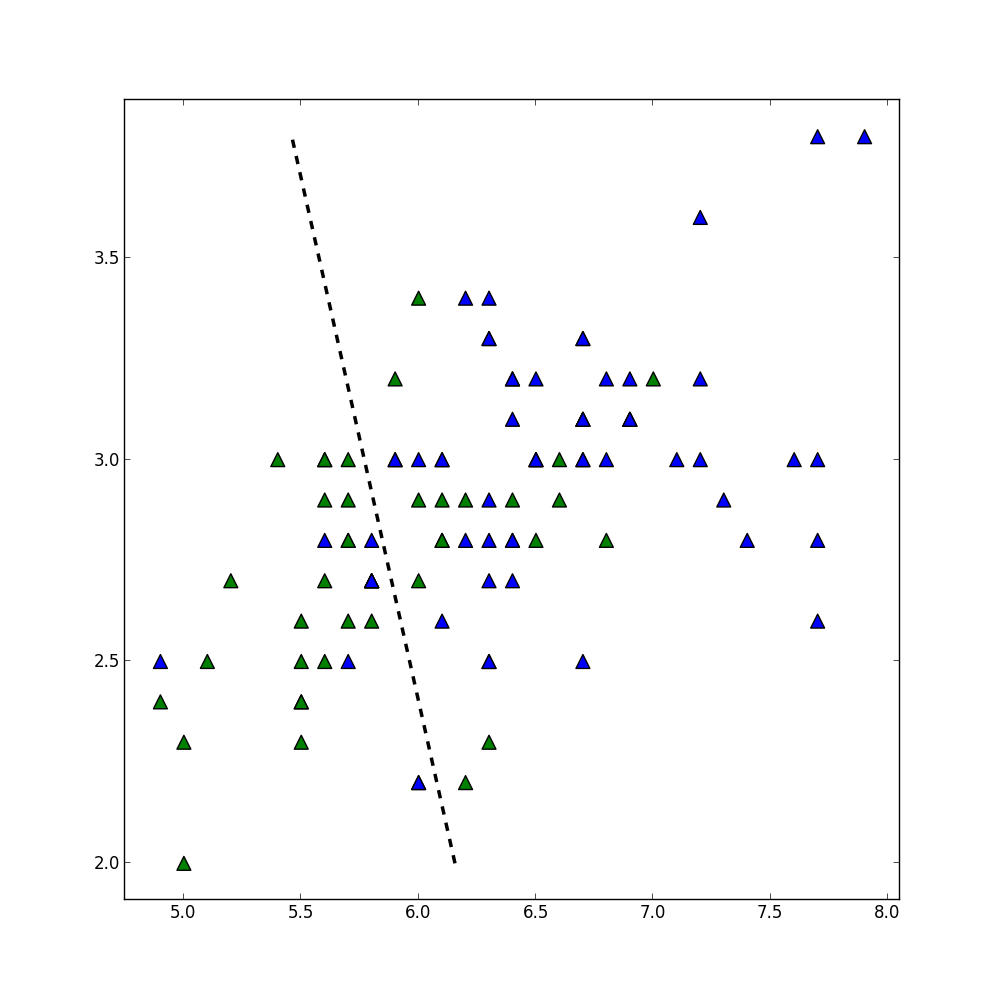
\includegraphics[scale=0.2]{images/lr12.png}
    \end{center}

\end{frame}

% ============================================== %

\section{Байесовский вывод}

% ============================================== %

\begin{frame}{Байесовский вывод}

\begin{block}{Дано}
\begin{itemize}
\item плотность вероятности $p(\mathbf{x} | \theta)$
\item априорная плотность $p(\theta)$
\item выборка $\mathbf{X} = \{x_1, \ldots, x_N\}$
\end{itemize}
\end{block}

\begin{exampleblock}{Найти}
апостериорную плотность $p(\theta | \mathbf{X})$
\end{exampleblock}

\[
p(\mathbf{x} | \mathbf{X}) = \int p(\mathbf{x} | \theta) p(\theta|\mathbf{X}) d\theta
\]

\[
p(\theta | \mathbf{X}) = \frac{p(\mathbf{X} | \theta) p(\theta)}{\int p(\mathbf{X} | \theta) p(\theta) d\theta}
\]

\[
p(\mathbf{X} | \theta) = \prod_n p(x_n | \theta)
\]

\end{frame}

% ============================================== %

\begin{frame}{Мультиклассовая классификация}

\begin{block}{Задача}
Использовать бинарный линейный классификатор для мультиклассовой классификации Ирисов. Какие идеи?
\end{block}

\vspace{1em}
Интерфейс классификатора  \texttt{clf}
\begin{itemize}
\item Использовать выборку $\mathbf{x}$, $\mathbf{y}$ для обучения \\ \texttt{\quad clf.fit(x, y)}
\item Предсказать класс объектов в $\mathbf{x}$ \\ \texttt{\quad y = clf.predict(x)}
\item Предсказать вероятности классов для $\mathbf{x}$ \\ \texttt{\quad y = clf.predict\_proba(x)}
\item Вычислить значение функции решения в $x$ \\ \texttt{\quad d = clf.decision\_function(x)}
\end{itemize}

\end{frame}

% ============================================== %

\begin{frame}{Домашнее задание 1}

\begin{block}{Линейные модели}
Реализовать на выбор
\begin{itemize}
\item Линейная классификация методом градиентного спуска
\item Линейная регрессия методом градиентного спуска
\item Линейная классификация инкрементальным методом
\item Линейная регрессия инкрементальным методом
\end{itemize}
\end{block}

Ключевые даты
\begin{itemize}
\item До 2014/03/14 23.59 выбрать задачу и ответственного в группе
\item До 2014/03/21 00.00 предоставить решение задания
\end{itemize}

\end{frame}

% ============================================== %

\begin{frame}{Спасибо!}

\begin{center}
{\Large Обратная связь}
\end{center}

\end{frame}

\end{document}